\documentclass[nobib]{tufte-handout}

\title{Pop-ups, politics,  NIMBYs \& legitimacy; lessons from failed bus lanes, Curitiba and Clarendon St}

\author{James Reynolds, PTRG, Monash University}

%\date{28 March 2010} % without \date command, current date is supplied

%\geometry{showframe} % display margins for debugging page layout

\usepackage{graphicx} % allow embedded images
  \setkeys{Gin}{width=\linewidth,totalheight=\textheight,keepaspectratio}
  \graphicspath{{graphics/}} % set of paths to search for images
\usepackage{amsmath}  % extended mathematics
\usepackage{booktabs} % book-quality tables
\usepackage{units}    % non-stacked fractions and better unit spacing
\usepackage{multicol} % multiple column layout facilities
\usepackage{lipsum}   % filler text
\usepackage{fancyvrb} % extended verbatim environments
\usepackage{natbib}
  \fvset{fontsize=\normalsize}% default font size for fancy-verbatim environments

% Standardize command font styles and environments
\newcommand{\doccmd}[1]{\texttt{\textbackslash#1}}% command name -- adds backslash automatically
\newcommand{\docopt}[1]{\ensuremath{\langle}\textrm{\textit{#1}}\ensuremath{\rangle}}% optional command argument
\newcommand{\docarg}[1]{\textrm{\textit{#1}}}% (required) command argument
\newcommand{\docenv}[1]{\textsf{#1}}% environment name
\newcommand{\docpkg}[1]{\texttt{#1}}% package name
\newcommand{\doccls}[1]{\texttt{#1}}% document class name
\newcommand{\docclsopt}[1]{\texttt{#1}}% document class option name
\newenvironment{docspec}{\begin{quote}\noindent}{\end{quote}}% command specification environment

\begin{document}

\maketitle% this prints the handout title, author, and date

\begin{abstract}
\noindent
This handout discusses \textbf{9 pragmatic strategies for implementation}\footnote{These are: (A) legitimisation before implementation through (A1) technical enquiry, (A2) transport planning, (A3) public processes; (B) avoiding impacts through (B1) grade-separation, (B2) additional capacity or (B3) subservience; and (C) legitimisation through implementation using (C1) bottom-up and incremental implementation, (C2) pop-ups and (C3) formal trials.} emerging from case study research. Politics, NIMBYs, reluctant institutions and other non-technical issues can have much influence on transport systems. Hence, transport policy-makers, -implementers and -researchers need to pay more attention to such issues\citep{Marsden:2017aa}. This handout briefly outlines recent research\citep{Reynolds:2020aa} responding to this call.  
\end{abstract}

%\printclassoptions

Why is improving transport so hard? What we might sometimes forget is that transport decisions are often made in council chambers, ministers' offices or by voters (most of whom are drivers), rather than by planners and engineers in technically-focused policy arenas.  \smallcaps{Legitimacy} comes in many forms\footnote{e.g. standards and laws state what 'should' be done and who 'shall' give way (normative legitimacy);  outputs of capacity analysis software may have legitimacy through trust; many impact assessment reports conclude 'the generated traffic can be reasonably accommodated on the existing road network' (legitimacy through reasonableness); and many are in favour of more bike/bus lanes, just not in their street (NIMBYism, related to legitimacy through conditional normative support)}. Engineers and planners might often be trained to find the 'best' solution, but that isn't necessarily the one that will be legitimate in the real world.   



\begin{marginfigure}%
  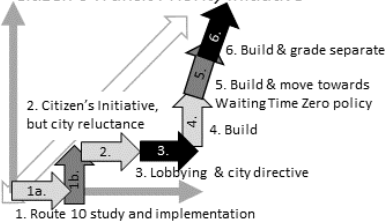
\includegraphics[width=\linewidth]{Zurich}
  \caption{Transit priority legitimacy and implementation in Zürich}
  \label{fig:Zurich}
\end{marginfigure}


The findings described here emerged from case study research, which generated a simple, two-axis framework (Figure 1) for understanding legitimacy and implementation. The x-axis indicates the \smallcaps{amount of transit priority that is legitimate}, while the y-axis denotes the \smallcaps{amount that exists}.  The framework's underlying premise is that, in the long-term,  x and y converge\footnote{Such that the amount that is provided is the amount that is legitimate. This is Indicated by the arrow showing x = y}. 

\newthought{Legitimacy before implementation} is what is shown in Figure 1 as having occurred in Zürich. In part this was through a \textbf{A1. technical report} that built legitimacy (Figure 1, arrow 1a) for installing (1b) tram priority measures on tram route. Importantly, this technical enquiry influenced broader public debate about transport in Zürich, in a similar way to how the City of Toronto provided technical results in a manner that was understandable to (and about things that mattered to) the public during the King Street Pilot (Figure 2). 
\begin{marginfigure}%
  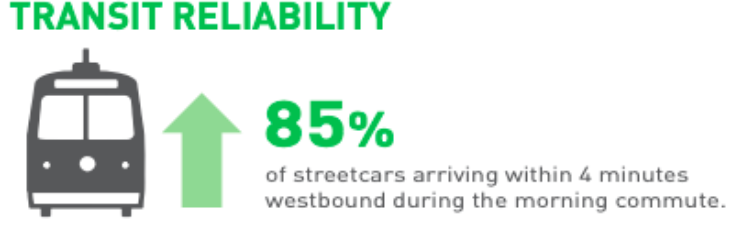
\includegraphics[width=\linewidth]{Toronto_dashboard_1}
   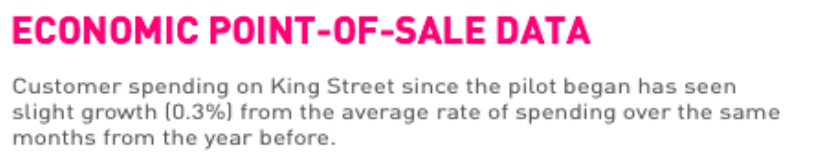
\includegraphics[width=\linewidth]{Toronto_dashboard_4}
  \caption{City of Toronto monthly dashboard during King Street Pilot, see thesis p.274}
  \label{fig:Toronto_dashboard}
\end{marginfigure}
It also helped in Zürich that when they adopted a \textbf{A2. Transport Plan} it was based on a vision for buses and trams to "travel along their lanes or tracks virtually as fast as is technically possible"\citep{Nash:2001ab}. Curitiba's famous Bus Rapid Transit (BRT) network was similarly led by a vision-based plan\footnote{The Plano Diretor, thesis chapter 8.}, for the city's transport and land-use to develop along linear 'Structural Axes'. This contrasts to the partially-removed Stud Road bus lanes here in Melbourne, for which the plan was objective-led\footnote{Namely, that there should be bus lanes along all of Stud Road.}.
The final pragmatic strategy for building legitimacy before implementation is \textbf{A3. Public Processes}, again perhaps best demonstrated by Zürich's Citizens' Transit Priority Initiative, which was narrowly passed in a public ballot\footnote{51\% for, 49\% against.  See Nash and Sylvia (2001) and thesis ch.7. Indicated in Figure 1 by arrow 2.}. Ballots appear rare, but the research found cases were council meetings, environmental assessment hearings and other public processes (including even court hearings) appear to have legitimised implementation.  

\newthought{But, why not simply avoid impacting} those who might oppose  implementation.  This approach was successful for the Eglinton Crosstown LRT in Toronto, some of which is \textbf{B1. Grade-separated} so as not to impact traffic. In the context of Mayor Rob Ford's declaration that "the war on the car is over" putting the trams underground was the only way to get transit priority (even though very expensive). Similarly,  the Stud Road bus lanes here in Melbourne were only removed where they had been converted from a traffic lane. Parts where they had been built as \textbf{B2. Additional Capacity} through road widening remain in place to this day.  \textbf{B3. Subservient priority} similarly seeks to limit opposition  by doing everything that can be done to help transit, but without impacting motorists, and is the genesis of Curibita's famous tubular bus stops and helps explains the retention of hook turns here in Clarendon Street. 

\begin{marginfigure}%
  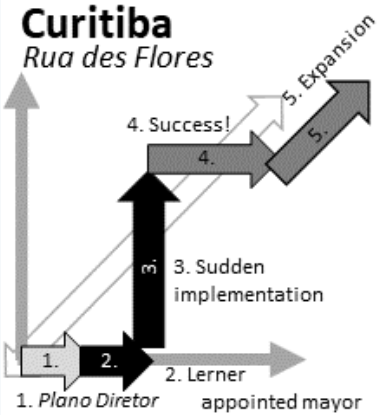
\includegraphics[width=\linewidth]{Curitiba_1}
    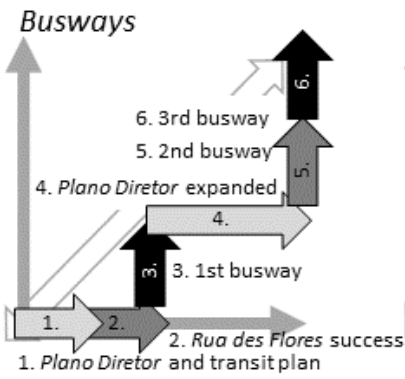
\includegraphics[width=\linewidth]{Curitiba_2}
        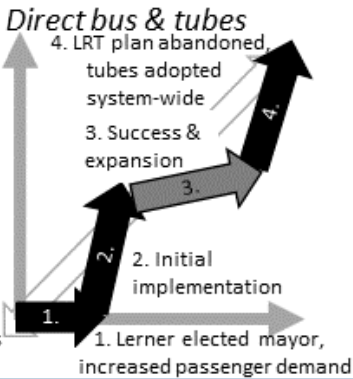
\includegraphics[width=\linewidth]{Curitiba_3}
  \caption{Progressions in Curitiba, thesis chapter 8}
  \label{fig:Curitiba}
\end{marginfigure}

\newthought{Legitimacy though implementation} relates to the idea that “if they had a chance to actually see it, everyone would love it”, as stated by Curitiba's Mayor, Jamie Lerner \citep{McKibben:2007aa}. With \textbf{C1. bottom-up and incremental implementation} successive small changes are made, building on initial successes (as in Curitiba). The gradual addition of tram separation kerbing in the Melbourne CBD over the last  approximately 20 years provides another example. \textbf{C2. Pop-ups} and \textbf{C3. Trials} provide other ways in which people can see what changes might look like in the real-world, without having to commit to permanence first.  For Jamie Lerner, it might help that he had the support of the military dictatorship ruling Brazil at the time his team converted central Curitiba into a pop-up pedestrian mall, but the guerrilla bike lanes of Seattle\citep{Fucoloro:2013aa} provide an example within democracies. At the least, as shown by Clarendon Street\citep{Silkstone:2005aa}, temporary implementations can be used to find out which measures actually are legitimate.

This two-page handout is not quite enough space to adequately squeeze in a 4-5 year PhD, 4 cases and an entire framework based on concepts from public policy analysis. Hopefully, though it might give you a start on some strategies for successfully improving transport systems in the real world of politics, NIMBYs and the other non-technical aspects of implementation. 

\bibliography{implementation_transit_priority_handout}
\bibliographystyle{plainnat}



\end{document}
